%% This is file `elsarticle-template-1-num.tex',
%%
%% Copyright 2009 Elsevier Ltd
%%
%% This file is part of the 'Elsarticle Bundle'.
%% ---------------------------------------------
%%
%% It may be distributed under the conditions of the LaTeX Project Public
%% License, either version 1.2 of this license or (at your option) any
%% later version.  The latest version of this license is in
%%    http://www.latex-project.org/lppl.txt
%% and version 1.2 or later is part of all distributions of LaTeX
%% version 1999/12/01 or later.
%%
%% Template article for Elsevier's document class `elsarticle'
%% with numbered style bibliographic references
%%
%% $Id: elsarticle-template-1-num.tex 149 2009-10-08 05:01:15Z rishi $
%% $URL: http://lenova.river-valley.com/svn/elsbst/trunk/elsarticle-template-1-num.tex $
%%
\documentclass[preprint,12pt]{elsarticle}

%% Use the option review to obtain double line spacing
%% \documentclass[preprint,review,12pt]{elsarticle}

%% Use the options 1p,twocolumn; 3p; 3p,twocolumn; 5p; or 5p,twocolumn
%% for a journal layout:
%% \documentclass[final,1p,times]{elsarticle}
%% \documentclass[final,1p,times,twocolumn]{elsarticle}
%% \documentclass[final,3p,times]{elsarticle}
%% \documentclass[final,3p,times,twocolumn]{elsarticle}
%% \documentclass[final,5p,times]{elsarticle}
%% \documentclass[final,5p,times,twocolumn]{elsarticle}

%% The graphicx package provides the includegraphics command.
\usepackage{graphicx}
%% The amssymb package provides various useful mathematical symbols
\usepackage{amssymb}

\usepackage{amsmath} % assumes amsmath package installed
\usepackage{amssymb}  % assumes amsmath package installed
\usepackage{mathrsfs}
\usepackage{float}
\usepackage{tikz}
\usepackage[spanish]{babel}
\selectlanguage{spanish}
\usepackage[utf8]{inputenc}
\usepackage{algorithm}
\usepackage[colorinlistoftodos]{todonotes}
\usepackage[colorlinks=true, allcolors=blue]{hyperref}
\usepackage[noend]{algorithmic}


    
%% The amsthm package provides extended theorem environments
%% \usepackage{amsthm}

%% The lineno packages adds line numbers. Start line numbering with
%% \begin{linenumbers}, end it with \end{linenumbers}. Or switch it on
%% for the whole article with \linenumbers after \end{frontmatter}.
\usepackage{lineno}

%% natbib.sty is loaded by default. However, natbib options can be
%% provided with \biboptions{...} command. Following options are
%% valid:

%%   round  -  round parentheses are used (default)
%%   square -  square brackets are used   [option]
%%   curly  -  curly braces are used      {option}
%%   angle  -  angle brackets are used    <option>
%%   semicolon  -  multiple citations separated by semi-colon
%%   colon  - same as semicolon, an earlier confusion
%%   comma  -  separated by comma
%%   numbers-  selects numerical citations
%%   super  -  numerical citations as superscripts
%%   sort   -  sorts multiple citations according to order in ref. list
%%   sort&compress   -  like sort, but also compresses numerical citations
%%   compress - compresses without sorting
%%
%% \biboptions{comma,round}

% \biboptions{}

\journal{Journal Name}

\begin{document}

\begin{frontmatter}

%% Title, authors and addresses

\title{Im\'agenes Biom\'edicas \\ Tareas II y III}

%% use the tnoteref command within \title for footnotes;
%% use the tnotetext command for the associated footnote;
%% use the fnref command within \author or \address for footnotes;
%% use the fntext command for the associated footnote;
%% use the corref command within \author for corresponding author footnotes;
%% use the cortext command for the associated footnote;
%% use the ead command for the email address,
%% and the form \ead[url] for the home page:
%%
%% \title{Title\tnoteref{label1}}
%% \tnotetext[label1]{}
%% \author{Name\corref{cor1}\fnref{label2}}
%% \ead{email address}
%% \ead[url]{home page}
%% \fntext[label2]{}
%% \cortext[cor1]{}
%% \address{Address\fnref{label3}}
%% \fntext[label3]{}


%% use optional labels to link authors explicitly to addresses:
%% \author[label1,label2]{<author name>}
%% \address[label1]{<address>}
%% \address[label2]{<address>}

\author{Joel Chac\'on Castillo}

\address{Guanajuato, M\'exico}
\end{frontmatter}

\section{ \textit{Thresholding Based on Attribute Similarity} - Umbralización Basado en la Similitud de Atributos}

Estos algoritmos realizan la selección de un valor de umbralización en base a algunos atributos de calidad o mediciones de similaridad entre la imágen original y la versión binaria de la imágen\cite{sezgin2004survey}.
%
Estos atributos pueden ser basados en la coincidencia de los bordes ``Edge Matching'',momentos en escala de grises, conectividad, textura, o estabilidad de los objetos segmentados.
%
Algunos otros algoritmos evalúan directamente la semejanza de las distribuciones de probabilidad acumulativa o la semejanza de una imágen original en escala de grises con una imágen binaria por medio de una medida difusa.

Particularmente, en el trabajo \citet{huang1995image} se propone un método donde se minimizá la una medida difusa de una imágen de entrada.
%
La función de pertenencia en este método de umbralización es utilizada para denotar la relación característica entre un pixel y su región de pertenencia (i.e. el objeto o el fondo).
%
Entre mayor sea la diferencia asoluta entre el objeto y el fondo menor es el valor de pertenencia.
%
Además, este método puede ser extendido fácilmente a umbralización multi-nivel. 


\subsection{\textit{The fuzzy set and membership function} - Conjunto difuso y función de pertenencia}

Sea $X$ un conjunto imágen de tamaño $M \times N$ con $L$ niveles, y $X_{mn}$ es el nivel de gris de un pixel $(m, n)$ en $X$.
%
Sea $\mu_x(X_{mn})$ un valor de pertenencia el cual representa el grado de poseer una cierta propiedad por el pixel $(m,n)$ en $X$; esto es, un sub-conjunto difuso del conjunto imágen $X$ puede ser escrito de la siguiente forma.
\begin{equation}
    X = \{ (X_{mn}, \mu_x(X_{mn}) )  \}
\end{equation}
donde $0 \leq \mu_x(X_{mn})\leq 1, m=0,1,...,M-1$  y $n=0,1,...,N-1$.
%
Particularmente, la función de pertenencia $\mu_X(X_{mn})$ puede comprenderse como una función característica que representa lo difuso de un pixel $(m,n)$ en $X$.
%
Para el propósito de umbralización de imágenes, cada pixel en la imágen debería poseer una relación cercana con su región de pertenencia, es decir, el objeto o el fondo.
%
Por lo tanto, el valor de pertenencia de un pixel en $X$ puede ser definido utilizando la relación entre el pixel y su región de pertenencia.
%

Así, siendo $h(g)$ el número de ocurrencias en un nivel de grises $g$ en una imágen de entrada.
%
Además, dado un valor de umbralización $t$, los niveles de gris promedio del fondo $\mu_0$ y el objeto $\mu_1$ pueden ser obtenidos como se indica a continuación.
%
\begin{equation}
    \mu_0 =  \sum_{g=0}^t g h(g) / \sum_{g=0}^t h(g)
\end{equation}
\begin{equation}
    \mu_1 =  \sum_{g=t+1}^{L-1} g h(g) / \sum_{g=t+1}^{L-1} h(g)
\end{equation}
%
Los promedios de cada nivel de gris $\mu_0$ y $\mu_1$, pueden ser considerados como los valores objetivo del fondo y el objeto dado un umbral $t$.
%
Así, la relación entre un pixel en $X$ y su región de pertenencia debería depender intuitivamente en la diferencia de su  nivel de gris y el valor objetivo de su región de pertenencia.
%
Por lo tanto, dejando la relación posea la propiedad de que cuanto menor sea la diferencia absoluta entre el nivel de gris de un pixel y su valor objetivo correspondiente, mayor será el valor de pertenencia del pixel.
%
Entonces,la función de pertenencia que realiza la evaluación de lo previamente mencionado para un pixel $(m ,n)$ se define a continuación.
%
\begin{equation}
\mu_x(X_{mn}) =
     \begin{cases}
             \frac{1}{1+|x_{mn} - \mu_0|/C} & si X_{mn} \leq t\\
             \frac{1}{1+|x_{mn} - \mu_1|/C} & si X_{mn} > t,
            
     \end{cases}
\end{equation}
donde $C$ es un valor constante (usualmente $C=g_{max} - g_{min}$) tal que $1/2 \leq \mu_x(X_{mn}) \leq 1$.
%
Para un umbral dado $t$, cualquier pixel en la imágen de entrada debería pertenecer ya sea al objeto o al fondo.
%
Por lo tanto, se espera que el valor de pertenencia para un pixel debería no ser menor que $1/2$.
%
La función de pertenencia propuesta refleja esta relación entre  un pixel y su región de pertenencia.
%
\subsection{\textit{Measures of Fuzziness} - Mediciones difusas}
La medición difusa indica un grado en el conjunto difuso, es decir es una función $f: A\longrightarrow\Re$.
%
Se han propuesto varios enfoques para medir lo difuso.
%
En este caso se introducen dos metodos popularmente utilizados.
%
El primero es la medición de la entropía por medio de la función de Shannon y otro es la medición de Yager's por medio de la distancia entre el conjunto difuso y su complemento.
%

\subsubsection{Entropía}
La entropía utilizada como una medición difusa se puede ver como una analogía con la entropía en teoría de la información, sin embargo una diferencia mu sutíl en la definición.
%
Basado en la función de Shannon, se define la entroía de un conjunto  difuso $A$ como se indica a continuación.
\begin{equation}
    E(A) = \frac{1}{n ln 2} \sum_i S(\mu_A(x_i)), \quad i =1, 2, ..., n,
\end{equation}
con la siguiente función de Shannon.
\begin{equation}
    S(\mu_A(x_i)) = - \mu_A(x_i) ln[ \mu_A(x_i) ] - [1-\mu_A(x_i)]ln[1-\mu_A(x_i)]
\end{equation}
Extendiendo al caso de dos dimensión de una imágen plana, la entropía de una imágen $X$ se expresa a continuación.
\begin{equation}
    E(X) = \frac{1}{MN ln 2} \sum_m \sum_n S(\mu_x(X_{mn}))
\end{equation}
con $m=0,1,...,M-1$ y $n=0,1,...,N-1$
Finalmente, utilizando la información del histograma, la medición pues ser vista de la siguiente forma.
\begin{equation}
    E(X) =\frac{1}{MNln2} \sum_g S(\mu_x(g)) h(g) \quad g=0,1,...,L-1
\end{equation}
Es importante notar que la función de Shannon es monóticamente creciente en el intérvalo $[0, 0.5]$ y decreciente en el intérvalo $[0.5, 1]$.
%
Así, cuando $\mu_x(X_{mn}) = 0.5$ para todos los pixeles, la entropía $E$ será máxima.

\subsubsection{Medición de Yager}
La mayor distinción entre el conjunto difuso y la tendencia tradicional es que el enfoque de conjuntos difusos no siempre satisface la ley de excluir el medio.
%
Así, Yager argumenta que la medición difusa debería depender en la relación que existe entre un conjunto difuso $A$ y su complemento $\overline{A}$.
%
La distancia entre el conjunto difuso de una imágen $X$ y su complemento $\overline{X}$ es definido como se indica a continuación.
\begin{equation}
    D_p(X, \overline{X}) = \left [  \sum_m \sum_n |\mu_x(X_{mn}) - \mu_{\overline{x}}(X_{mn})|^p  \right ] ^{\frac{1}{p}}
\end{equation}
donde $\mu_x(X_{mn}) = 1-\mu_x(X_{mn})$. 
%
Por lo tanto, la medición difusa de $X$ puede ser denotada como:
\begin{equation}
    \eta_p(X) = 1 - \frac{D_p(X,\overline{X}}{|X|^{\frac{1}{p}}} = 1 - \frac{D_p(X,\overline{X}}{(MN)^{\frac{1}{p}}}
\end{equation}
Para simplificar los cálculos, se puede utiliza el histograma de la siguiente forma:
\begin{equation}
    D_p(X, \overline{X}) = \left [ \sum_g | \mu_x(g) - \mu_{\overline{x}}(g) |^p \right ] ^{\frac{1}{p}} h(g)
\end{equation}
Es importante notar que para $p=1$ se utiliza la métrica de hamming, y para $p=2$ es considerada la métrica Euclidieana.
%
Así, para una imágen $X$, se espera que la medición difusa debería ser tan pequeña como sea posible.
%


\section{\textit{A Threshold Selection Method from Gray-Level Histograms} - Un Método para la Selección de Umbrales Basado en Histogramas de Escalas de Grises (Otsu)}

En este trabajo se presenta un método automático y no-paramétrico para la selección de un umbral cuyo propósito es la segmentación de imágenes propuesto por \citet{otsu1979threshold}.
%
El procedimiento automatizado para la selección del umbral óptimo es seleccionado en base a el criterio discriminante, donde se desea maximizar la separabilidad de las clases resultantes en escala de grises.
%
El procedimiento es muy simple, y además utiliza el primer momento acumulativo (media acumulativa) del histograma en escala de grises.
%
Dados los pixels de una imágen y representados en escalas de grises $[1,2,...,L]$.
%
El número de pixeles en el nivel $i$ es denotao por $n_i$ y el número total de pixeles por $N=n_1+n_2+...n_L$.
%
Además, el histograma en escala de grises es normalizado y representado como una distribución de probabilidad:
\begin{equation}
    p_i = n_i/N \quad p_i \geq 0, \quad \sum_{i=1}^L p_i=1
\end{equation}

Así, en basea un umbral $k$ se separan los pixeles en dos clases $C_0$ y $C_1$ (fondo y objectos de interés).
%
Donde $C_0$ denota los pixeles con niveles $[1,...,k]$, y $C_1$ denota los pixeles con niveles $[k+1,...,L]$.
%
Entonces, la probabilidad de ocurrencia de cada clace y las medias de cada clase son indicados de la siguiente forma:
\begin{equation}
    \omega_0 = Pr(C_0) = \sum_{i=1}^k p_i = \omega(k)
\end{equation}
\begin{equation}
    \omega_1 = Pr(C_1) = \sum_{i=1}^k p_i = 1-\omega(k)
\end{equation}
\begin{equation}
    \mu_0 = \sum_{i=1}^k i Pr(i|C_0) = \sum_{i=1}^k i p_i / \omega_0 = \mu(k)/\omega(k)
\end{equation}
\begin{equation}
    \mu_1 = \sum_{i=k+1}^L i Pr(i|C_1) = \sum_{i=k+1}^L i p_i / \omega_1 = \frac{\mu_T - \mu(k)}{1-\omega(k)}
\end{equation}
donde
\begin{equation}
  \begin{split}
    \omega(k) &= \sum_{i=1}^k  p_i \\
    \mu(k) &= \sum_{i=1}^k i p_i
  \end{split}
\end{equation}
corresponden al acumulativo del cero y primer momento respectivamente del histograma generado por el umbral $k$.
%
Además, $\mu_T = \mu(L) = \sum_{i=1}^L i p_i$ es la media total de la escala de grises que pertenece a la imágen.
%
Así, se puede verificar la siguiente relación para cualquier orden $k$
\begin{equation}
    \omega_0 \mu_0 + \omega_1 + \mu_1 = \mu_T, \quad \omega_0 + \omega_1 = 1
\end{equation}

Las varianzas o momentos acumulativos de segundo orden de cada clase son determinados de la siguiente forma:
\begin{equation}
    \sigma_0 ^2 = \sum_{i=1}^k (i-\mu_0)^2 Pr(i | C_0) = \sum_{i=1}^k (i-\mu_0)^2  p_i / \omega_0
\end{equation}
\begin{equation}
    \sigma_1 ^2 = \sum_{i=1}^k (i-\mu_1)^2 Pr(i | C_1) = \sum_{i=k+1}^L (i-\mu_1)^2  p_i / \omega_1
\end{equation}

Así, para cualificar un determinado umbral se utiliza un criterio de medición del discriminante (i.e. mide la separabilidad de las clases):
\begin{equation}
    \lambda = \sigma_B^2/\sigma_W^2, \quad k = \sigma_T^2/\sigma_W^2, \quad \eta = \sigma_B^2/\sigma_T^2,
\end{equation}
donde
\begin{equation}
    \begin{split}
        \sigma_w^2 &= \omega_0 \sigma_0^2 + \omega_1 \sigma_1^2 \\
        \sigma_B^2 &= \omega_0(\mu_0 - \mu_T)^2 + \omega_1(\mu_1 - \mu_T)^2 \\
        &= \omega_0 \omega_1(\mu_1 - \mu_0)^2
    \end{split}
\end{equation}
Además se tiene que $\sigma_T^2 = \sum_{i=1}^L (i-\mu_T)^2 p_i$, es decir $\sigma_w$ es la varianza intra-clase y $\sigma_T$ es la varianza entre-clases.
%
De esta forma el problema se convierte en uno de optimización donde se obtenga el umbreal $k$ el cual maximiza cualquier critero de medición $\lambda, K, \eta$.
%
El criterio par discriminar basado en la maximización de $\lambda, K, \eta$ para un $k$ son equivalentes, es decir, basta con maximizar uno dada la siguiente relación básica:
\begin{equation}
    \sigma_w^2 + \sigma_B^2 = \sigma_T^2
\end{equation}
Se puede observar que $\sigma_w^2$ y $\sigma_B^2$ son función del umbral $k$, pero $\sigma_T^2$ es independiente de $k$.
%
Además, $\sigma_w^2$ se basa en estadísticas de segundo orden (varianza de las clases), mientas $\sigma_B^2$ se basa en la estadística de primer orden (media de las clases).
%
Por lo tanto, $\eta$ es la medición más simple con respecto al umbral.
%
Entonces, se utiliza $\eta$ como un criterio de medición para medir la calidad de separación dado un umbral $k$.
%

El umbral óptimo $k^*$ el cual maximiza $\eta$, o equivalentemente, el que maximiza $\sigma_B^2$ es seleccionado en base a una búsqueda secuencial utilizando $\eta(k) = \sigma_B^2(k)/\sigma_T^2$.
%
Por lo tanto el umbral óptimo $k^*$ es determinaod en base a la siguiente función objetivo:
\begin{equation}
    \sigma_B^2 (k^*) = max_{1 \leq k < L} \quad \sigma_B^2(k)
\end{equation}
Así, la función objetivo que corresponde a la forma generalizada o multi-clase se puede representar como sigue:
\begin{equation}
    \begin{split}
        \sigma_B^2( k_1^*, ..., k_{NC}^*) &= arg \quad max_{1\leq k_1,...,k_{Nc}} \quad  \sum_{i=1}^{NC} \omega_i (\mu_i - \mu_T)^2 
    \end{split}
\end{equation}
donde $NC$ es el número de clases que se desean separar en la imágen.

\section{\textit{A New Method for Gray-Level Picture Thresholding Using the Entropy of the Histogram} - Un Nuevo Método para el Umbral de Imágenes de Nivel de Gris Mediante la Entropía del Histograma}

Los método más comúnes para la extracción de objetos de una imágen son basados en un umbral.
%
Si el objeto se distingue de forma clara del fondo, sin embargo el histograma que pertenece a la imágen en escala de grises no siempre posee el comportamiento de bimodalidad.
%
En base a este inconveniente \citet{pun1980new} propone utilizar el ratio entre la entropía a posteriori $H^\prime_n$ y la entropía $H_n$ que es acotada por un funcional $f(s)$, definidos de la siguiente forma.
\begin{equation}
    H^\prime_n = -P_s ln P_s -(1-P_s) ln (1-P_s)
\end{equation}
donde $P_s = \sum_{i=1}^s p_i$, $1-P_s = \sum_{i=s+1}^n p_i$ 
%
por su parte la entropía se define de la siguiente forma
\begin{equation}
    H_n = -\sum_{i=1}^n p_i ln p_i
\end{equation}
%
El resultado más importante de ese trabajo es establecer la siguiente relación
\begin{equation}
    \left (\phi(s) = \frac{H^\prime_n}{H_n} \right ) \leq f(s)
\end{equation}
donde argumentan que $f(s)$ mayoriza $\phi(s)$ asumiendo un error como se observa en la siguiente imágen.
%
\begin{figure}[H]
\centering
\begin{tabular}{c}
   \includegraphics[width=0.5\textwidth]{entropy.png}  
\end{tabular}
\caption{Relación entre el funcional $f(s)$ y el ratio de entroías $\phi(s)$ .}
\end{figure}

Por otra parte varios años después \citet{kapur1985new} demostraron que el funcional $f(s)$ tenía inconvenientes importantes:
\begin{itemize}
    \item La maximización de $f(s)$ no logra una maximización a priori de una entropía a posteriori $H^\prime_n$..
    \item Desde que $H^\prime_n$ es mayorizada por otra función, el algoritmo no utiliza las propiedades estadísticas del histograma de escalas de grises.
\end{itemize}
%
Por lo tanto \citet{kapur1985new} proporcionan un enfoque el cual se basa en la sumatoria de las entropías obtenidas por cada clase como se indica a continuación.
%
Dadas las distribución en escala de gris $p_1, p_2, ..., p_n$ y dado un umbral $s$ (se utiliza la misma notación que en el trabajo propuesto), se derivan dos distribuciones de probabilidad de la siguiente forma.
\begin{equation}
    A: \frac{p_1}{p_s}, \frac{p_2}{p_s}, ..., \frac{p_s}{p_s}
\end{equation}
\begin{equation}
    B: \frac{p_{s+1}}{1-p_s}, \frac{p_{s+2}}{1-p_s}, ..., \frac{p_{n}}{1-p_s}
\end{equation}
Además, la entropías asociadas con cada distribución se definen a continuación:
\begin{equation}
   \begin{split}
    H(A) &= - \sum_{i=1}^s \frac{p_i}{P_s} ln\frac{p_i}{P_s} \\
    &= -\frac{1}{P_s} \left [ \sum_{i=1}^s p_i ln p_i - p_i ln P_s  \right ] \\
    &= ln P_s + \frac{H_s}{P_s}
   \end{split}
\end{equation}
similarmente:
\begin{equation}
   \begin{split}
    H(B) &= - \sum_{i=1+s}^n \frac{p_i}{1-P_s} ln\frac{p_i}{1-P_s} \\
    &= -\frac{1}{1-P_s} \left [ \sum_{i=1+s}^n p_i ln p_i - (1-p_i) ln(1-P_s)  \right ] \\
    &= ln (1-P_s) + \frac{H_n - H_s}{1-P_s}
   \end{split}
\end{equation}
Entonces definiendo la suma de $H(A)$ y $H(B)$ como $\phi(s)$:
\begin{equation}
    \phi(s) = ln P_s (1-P_s) + \frac{H_s}{P_s} + \frac{H_n - H_s}{1-P_s}
\end{equation}
Por lo tanto se desa maximizar $\phi(s)$ para obtener la máxima informaión entre la distribución del objeto y la distribución del fondo en la imágen.
%
La forma multi-nivel se obtiene maximizando la siguiente función objetivo
\begin{equation}
    \phi(s_1^*, ..., s_k^*) = \max_{s_1,...,s_k} \quad \sum_{i=1}^k H(X_i)
\end{equation}
donde $k$ es el número de niveles que se desean identificar.

\section{Indicadores de Calidad}\label{sec:4}

En el análisis de imágenes médicas es necesario identificar o segmentar estructuras de su fondo.
%
Es importante entender que no existe una técnica universal de segmentación para lidiar con todo tipo de imágenes médicas.
%
Por lo tanto, encontrar una algoritmo de segmentación para una específica tarea como elegir los parámetros óptimos aún es un reto.
%
Por otra parte, escoger una medición de la efectividad dado un algoritmo aún es una tarea difícil.
%
Sin embargo, se presentan cinco métricas popularmente consideradas~\cite{fenster2006evaluation}

\subsection{Accuracy}
La exactitud de una técnica de segmentación se refiere al grado en el cual los resultados dado un método de segmentación concuerdan con el resultado de segmentación real.
%
Así, esta métrica se encarga de medir la proporción de positivos y negativos que fueron correctamente indetificados por un clasificador.
%
El dominio de esta métrica es $[0,1]$, donde $0$ es la peor clasificación y $1$ es la mejor clasificación.
%
\begin{equation}
    Acccuracy = \frac{TP + TN}{(TP + FP + TN +FN)}
\end{equation}
\subsubsection{Sensitivity - \textit{True Positive Rate or True Positive Fraction}}
Se encarga de medir la proporción de positivos que fueron correctamente identificados por algún clasificador.
%
Se encuentra definida en el intérvalo $[0,1]$, donde $0$ es la peor clasificación y $1$ es la clasificación perfecta.
\begin{equation}
    Sensitivity = \frac{TP}{(TP+ FN)}
\end{equation}

\subsection{Specificity - \textit{True Negative Rate or True Negative Fraction}}
Se encarga de medir la proporción de negativos que fueron correctamente identificados por algún clasificador. 
%
El dominio de esta métrica es $[0, 1]$ donde $0$ es la peor clasificación y $1$ es la clasificación perfecta.
\begin{equation}
    Specificity =  \frac{TN}{(TN + FP)}
\end{equation}

\subsection{Positive Predictive Value - PPV}
Mide la proporción de positivos que fueron correctamente e incorrectamente identificados por un clasificador.
%
Está definido en el dominio $[0, 1]$, donde $0$ es la peor clasificación y $1$ es la clasificación perfecta.
\begin{equation}
    PPV = \frac{TP}{(TP + FP)}
\end{equation}
\subsection{Negative Predictive Value - NPV}
Mide la proporción de negativos que fueron correctamente identificados por algún clasificador.
%
Está definido en el intérvalo $[0, 1]$, donde $0$ es la peor clasificación y $1$ es la clasificación perfecta.
\begin{equation}
    NPV = \frac{TN}{(TN + FN)}
\end{equation}

\section{Evolución Diferencial en problemas de imágenes}

Evolución Diferencial (ED) fue inicialmente propuesto por \citet{price2006differential}, sin embargo en este mismo trabajo se explica que este algoritmo es una variante aleatorizada del algoritmo ``Nelder Mead'' \cite{olsson1975nelder}.
%
Esta sección está dedicada a revisar la variante clásica de DE y a introducir varios términos importantes que son utilizados en el campo de DE.
%
DE es un algoritmo estocástico basado en una población, por lo que en cada instante maneja un conjunto de soluciones candidatas que van evolucionando de forma iterativa.
%
En DE dichas soluciones candidatas son usualmente conocidas como vectores.
%
En la variante básica de DE, para cada miembro de la población (conocidos como \textit{vectores objetivo}) se genera un nuevo vector que es conocido como el \textit{vector mutado}.
%
A continuación, el vector mutado se combina con el vector objetivo para generar al \textit{vector de prueba} y finalmente se procede con la fase de selección para elegir a los vectores sobrevivientes.
%
De esta forma, las generaciones transcurren de forma iterativa hasta cumplir el criterio de paro.
%
Así, el $i$-ésimo vector de la población en la generación $G$ se denota como$\vec{X}_{i,G} = [x_{1,i,G}, x_{2,i,G},..., x_{D,i, G}]$.
%
A continuación se explica en más detalle cada componente de DE.

\subsubsection{Inicializaci\'on}

Usualmente, DE inicia el proceso de optimización con una población de $NP$ vectores que son creados de forma aleatoria.
%
Habitualmente los vectores de la población inicial son generados en base a una distribución uniforme, ya que usualmente no se posee información sobre cuáles son las zonas más promisorias del espacio de búsqueda.
%
Por lo tanto, el $j$-ésimo componente del $i$-ésimo vector es inicializado de la forma $x_{j,i,0} = x_{j}^{(L)} + rand_{i,j}[0,1] (x_{j}^{(U)} - x_{j}^{(L)})$,
donde $rand_{i,j}[0,1]$ es un número aleatorio uniformemente distribuido entre $0$ y $1$.

\subsubsection{Operador de mutaci\'on}

Por cada vector objetivo se genera un vector mutado para lo cual se han propuesto múltiples estrategias con la particularidad de que en cierta forma
se usen las diferencias entre vectores.
%
La variante clásica de DE aplica la estrategia conocida como rand/1, en la cual se crea un vector mutado $V_{i,G}$ de la siguiente forma:

\begin{equation}\label{eqn:mutation}
\vec{V}_{i,G} = \vec{X}_{r1, G} + F \times (\vec{X}_{r2, G} - \vec{X}_{r3, G}) \quad r1 \neq r2 \neq r3
\end{equation}

En la Ecuación~(\ref{eqn:mutation}) los índices $r1, r2, r3 \in [1,NP]$ deben ser enteros distintos y son generados de forma aleatoria
en el rango $[1, NP]$.
%
Además, estos índices son distintos al índice $i$.
%
Es importante hacer notar que la diferencia entre los vectores es escalada por medio del parámetro $F$, el cual usualmente se define en el intervalo $[0.4, 1]$.
%
Posteriormente, el vector de diferencia (escalado) es agregado a un tercer vector, lo que significa que los vectores mutados son similares a los vectores objetivo si el grado de diversidad es bajo, ya que los vectores de diferencias tienen norma pequeña.
%
Como consecuencia de esto es claro que es crítico mantener un grado mínimo de diversidad en DE.

\subsubsection{Operador de cruce}

El operador de cruce se aplica con el objetivo de combinar la información de distintas soluciones candidatas y de incrementar la diversidad de los vectores.
%
Específicamente, cada vector objetivo $\vec{X}_{i,G}$ se mezcla con su correspondiente vector mutado $V_{i,G}$ para generar un vector de prueba $\vec{U_{i,G}} = [u_{1,i,G},u_{2,i,G}, ..., u_{D,i,G} ]$.
%
La estrategia de cruce mas típica es conocida como \textit{cruce binomial} y actúa de la siguiente forma:

\begin{equation} \label{eqn:crossover}
\vec{U}_{j,i,G}= 
\begin{cases}
    \vec{V}_{j,i,G},& \text{si} \quad (rand_{i,j}[0,1] \leq CR \quad o \quad j = j_{rand}  )\\
    \vec{X}_{j,i,G},              & \text{de otra forma}
\end{cases}
\end{equation}

En la Ecuación~(\ref{eqn:crossover}) $rand_{i,j}[0,1]$ es un número uniformemente distribuido, 
$j_{rand}$ es un índice seleccionado aleatoriamente que asegura que $\vec{U}_{i,G}$ genera al menos un componente 
de $\vec{V}_{i,G}$ y $CR \in [0,1]$ es la razón de cruce.
%el ratio de cruce.

\subsubsection{Operador de selección}
Finalmente, se aplica una selección elitista para determinar los vectores sobrevivientes que participarán en la siguiente generación.
%
Específicamente, cada vector de prueba se compara con su correspondiente vector objetivo y sobrevive el que tiene la mejor aptitud:

\begin{equation} \label{eqn:selection}
\vec{X}_{j,i,G+1}= 
\begin{cases}
    \vec{U}_{i,G},& \text{si} \quad f(\vec{U}_{i,G}) \leq f(\vec{X}_{i,G})  \\
    \vec{X}_{i,G},              & \text{de otra forma}
\end{cases}
\end{equation}

Debido a la forma de seleccionar a los sobrevivientes en cada generación los miembros de la población permanecen iguales o mejoran.
%
Por ello, se considera que DE hace uso de una selección muy elitista y es una de las razones por la que en ciertos casos puede sufrir de una convergencia demasiado acelerada.

\subsection{Adaptación de Evolución Diferencial en un problema discreto}
Particularmente, se desea utilizar DE en un problema de optimzación discreto donde el conjunto factible está comprendido de  únicamente números enteros y los límites inferior y superior  son $x^{(L)}=0$ y $x^{(U)}=254$ respectivamente.
%
Inicialmente, se podría considerar la variante estándar de Evolución Diferencial donde el resultado (contínuo) es redondeado a un entero.
%
Sin embargo, esto puede crear problemas de conergencia, e inclusive --dependiendo del problema-- podría generar platos \textit{platus}, es decir, cambios en el espacio de la variables no tienen efectos en el espacio objetivo por lo tanto el proceso de búsqueda podría estancarse.
%

En la versión de Evolución Diferencial propuesta en este trabajo se utilizan una modificación tanto del operador de mutación como el operador de cruce.
%
\textbf{La principal ventaja de esta propuesta es que no requiere tanto el parámetro de escala $F$ como la probabilidad de mutación $CR$ }.
%

\subsection{Operador de mutación propuesto para este problema discreto}

En las variantes más recientes de Evolución Diferencial se prefiere utilizar una distribución de probabiliadad en $F=Normal(0.5, 0.1)$, esto en base a que ED tiene un comportamiento de búsqueda más adecuado.
%
En este caso, en lugar de utilizar un factor de escala se considera una distribución uniforme discreta en el intérvalo $[1, \vec{X}_{r2, G} - \vec{X}_{r3, G}]$.

\begin{equation}
\begin{split}
&\vec{V}_{i,G} = \vec{X}_{r1, G} +  signo(Diff) \times randint( 1, abs(Diff)) \quad r1 \neq r2 \neq r3   
\end{split}
\end{equation}
donde $Diff = \vec{X}_{r2, G} - \vec{X}_{r3, G}$.
%
En este problema discreto, este procedimiento es válido a pesar de que el dominio es discreto, el espacio factible está comprendido por una especie de cono, es decir, todos los vecinos de un pixel (dentro del hyper-cubo del espacio factible) poseen un mapeo directo al espacio objetivo.

\subsection{Operador de cruce propuesto para este problema discreto}
En la literatura se argumenta que Evolución Diferencial resuelve un problema continuo discretizándolo.
%
Una de las principales razones por las cuales se considera ED como un problema discreto, es que selecciona los componentes de un vector y el tamaño en base a una distribución binomial la cual modifica su comporamiento en base a la probabilidad de cruce.
%
Entre mayor sea la probabilida de cruce, mas elementos serán modificados.
%
Una forma para evitar que asignar este parámetro es mediante un esquema adaptativo como lo hacen los algoritmos Shade \cite{tanabe2013success}.
%
En este caso se opta por utilizar una probabilidad de cruce en base a una distribución uniforme $CR = U[0,1]$, es decir, en algunos casos se cambian más elementos que en otros.
%
Es importante notar que siempre se va a modificar al menos un valor en cada cruce, por lo tanto si $CR=0$ no causara vectores iguales.

\begin{equation} 
\vec{U}_{j,i,G}= 
\begin{cases}
    \vec{V}_{j,i,G},& \text{si} \quad (rand_{i,j}[0,1] \leq CR \quad o \quad j = j_{rand}  )\\
    \vec{X}_{j,i,G},              & \text{de otra forma}
\end{cases}
\end{equation}

\section{Problema de Combinatoria para Umbralizar a varios niveles}

Los métodos multi-nivel considerados en este trabajo fueron programados para calcular cualquier número de clases.
%
La manera de realizar esto fue por medio de un método recursivo el cual resuelve un problema bien conocido en la literatura del ámbito de programación, es decir encontrar todas las combinaciónes dado un conjunto factible.
%
Para mayor información se puede visitar el libro \citet{cormen2009introduction}.


\section{Validación Experimental}

La parte experimental se enfoca en medir distintas propiedades de los siguientes variantes previamente explicadas:
\begin{itemize}
    \item El método de Otsu.
    \item El método de Kapur.
    \item El método de difuso con entropía.
    \item Variante de Otsu optimizada con Evolución Diferencial (ED).
    \item Variande te Otsu optimizada con descenso de gradiente y diferencias finitas.
\end{itemize}

\subsection{Eficiencia en relación de los métodos propuestos}
Es importante notar que todos los métodos propuestos (incluyendo Otsu y Kapur) utilizan el mismo paradigma considerado en imágenes integrales \cite{viola2004robust}.
%
Este principio consiste en pre-calcular una tabla acumulativa como se muestra en la siguiente tabla:
\begin{table}[H]
\centering
\begin{tabular}{|c|c|c|c|c|c|c|}
\hline
1 & 2 & 3 & 4 & 5 & 6 & 7 \\ \hline
x\_i & $\sum_{i=1}^2 x_i$ & $\sum_{i=1}^3 x_i$ & $\sum_{i=1}^4 x_i$ & $\sum_{i=1}^5 x_i$ & $\sum_{i=1}^6 x_i$ & $\sum_{i=1}^7 x_i$ \\ \hline
\end{tabular}
\end{table}
Así, si se desea la sumatoria entre $x_4$ y $x_6$ solo se tendría que calcular la diferencia el valor de la sumatoria que pertenece a la casilla 6 - el valor de la sumatoria que pertenece a la casilla 3, proporcionando consultas en tiempo constante $O(c)$ en lugar de tiempo lineal $O(n)$.

\subsection{Umbralización de Imágenes considerando dos clases}

En esta sección se presentan los resultados obtenidos de aplicar los métodos previamente explicados.
%
Para llevar esto, se consideran las métricas explicadas en la sección \ref{sec:4}, donde el proceso de medición consiste en contabilizar los valores $TP$, $TN$, $FP$ y $FN$ de todas las imágenes y tomar las métricas en base a estos valores.
%
Esto sería equivalente a generar una imágen grande la cual está construída de todo el conjunto de mágenes de prueba.
%
Además, se calcular la media obtenida con cada algoritmo, es decir, se consideran las métricas de forma individual en cada imágen.
%
La media sirve para verificar si la calidad de un experimento (una imágen) es muy malo, entonces se podrían comparar los  resultados al considerar los resultados de la imágen grande (consiste en juntar todas las imágenes) con la media.
%
Este conjunto consta de $30$ imágenes, las cuales aunque no cuentan con su \textit{grand-truth}, sin embargo posee un las coordenadas de los objetos de  interés.
%
En base a esto, para obtener el \textit{grand-truth} se utiliza un algoritmo recursivo (backtracking) el cual dada la coordenada de un pixel visita a los pixeles vecinos y si poseen la misma intensidad en escala de grises  que el pixel principal son considerados como pixeles de interés.
%
Para todos los experimentos, el algoritmo basado en evolución diferencial utiliza una población de tamaño $10$ y un número  de $50$ generaciones.
%
Principalmente, se puede observar que la función objetivo (enfoque de Otsu) no proporciona una fórmula directa para calcular el gradiente respecto a un umbral determinado.
%
Por lo tanto para realizar el cálculo del gradiente se utilizan diferencias finitas centrales (se tuvo que probar con distintos tamaños de paso se que con $\alpha > 0.5$).
%
Adicionalmente, se considera la variante de Otsu proporcionada por la librería \textit{skimage}.
%
En la tabla \ref{tab:1} se presentan los resultados de los seis algoritmos, donde en las primeras cuatro columnas se pueden observar los resultados al considerar una imágen grande (generada por todas las imágenes) y en las últimas cuatro columnas se presenta se presenta la medie de considerar una métrica en cada imágen de forma individual.
%
Se puede observar que la sensibilidad es mejor con el método de Kapur, la razón de esto es que el método de Kapur resalta una mayor región de interés.
%
Particularmente, la sensibilidad únicamente mide el grado en que se obtuvo el objeto de interés, la desventaja de esta métrica es el caso extremo en que toda la  imágen sea identificada como objeto de interés, en resultado se tiene una métrica no fiable.
%
Este inconveniente, también surge con la especificidad.
%
La variante de Otsu que considera el gradiente obtiene mejores resultados en la especifidad, exactitud e índice de Jaccard.
%
Esto indica algo muy importante, es decir, a pesar de que la función a optimizar se basa la misma función objetivo que la del Otsu estándar esté algoritmo obtuvo mejores resultados.
%
La principal razón de esto es que el método de gradiente no siempre llagaba al óptimo global, es decir, depende totalmente del tamaño de paso.
%
Esto indica que la función objetivo representada por el método de Otsu puede tener problemas de sobre-ajuste.
%
Además es bien conocido en la literatura que la estimación de la varianza tiene problemas de sobre-ajuste, en resultado se puede ver que aunque los optimizadores puedan alcanzar el óptimo la calidad del resultado dependerá totalmente de la función objetivo.
%
Un punto interesante, es que al considerar el gradiente de la imagen el método de gradiente considera una versión simplificada del filtro de Sobel.

Por otra parte se observa que tanto el método de Otsu estándar como el método de Otsu con evolución diferencial proporcionan los mismos resultados en todos los indicadores, por lo tanto se puede establecer que la versión de evolución diferencial propuesto alcanza el óptimo en todas las imágenes.


En la imágen \ref{img:20} se observa que el método del gradiente (fila 2 derecha) y el que considera la función difusa con entropía \textit{fuzzy-entropy} (fila 3 izquierda) se aproximan más al objeto de interés.
%
Por otra parte en la imágen \ref{img:25} se observa que el método del gradiente (fila 2 derecha) proporciona los peores resultados.
%
Sin embargo el algoritmo que proporciona la función difusa con entropía representa de una mejor forma al objeto de interés.

% Please add the following required packages to your document preamble:
% \usepackage{graphicx}
\begin{table}[H]
\resizebox{\textwidth}{!}{%
\begin{tabular}{|c|c|c|c|c|c|c|c|c|}
\hline
\textbf{} & \textbf{Sensitivity} & \textbf{Specifity} & \textbf{Accuracy} & \textbf{Jaccard-Index} & \textbf{Mean-Sensitivity} & \textbf{Mean-Specifity} & \textbf{Mean-Accuracy} & \textbf{Mean-Jaccard-Index} \\ \hline
\textbf{Fuzzy-Entropy} & 0.9141733212 & 0.9706934158 & 0.9692271815 & 0.4352382467 & 0.9507412794 & 0.9708051953 & 0.9692271815 & \textbf{0.436446802} \\ \hline
\textbf{Otsu} & 0.9966280877 & 0.8716180531 & 0.8748670474 & 0.1714980051 & 0.9989194673 & 0.8730104869 & 0.8745987932 & 0.3286984941 \\ \hline
\textbf{Otsu-DE} & 0.9966280877 & 0.8716180531 & 0.8748670474 & 0.1714980051 & 0.9989194673 & 0.8730104869 & 0.8745987932 & 0.3286984941 \\ \hline
\textbf{Otsu-Gradient} & 0.9557967515 & \textbf{0.9736502483} & \textbf{0.9731870015} & \textbf{0.4805008691} & 0.8654891558 & \textbf{0.973310246} & \textbf{0.9731825563} & 0.4123111584 \\ \hline
\textbf{Otsu-skimage} & 0.9969660354 & 0.8576350713 & 0.8612584233 & 0.1574468336 & \textbf{0.9990275792} & 0.8591676934 & 0.8609691471 & 0.2899804435 \\ \hline
\textbf{Kapur} & \textbf{1} & 0.8362011413 & 0.8404741328 & 0.1405443855 & 1 & 0.837969414 & 0.8405240775 & 0.2177993445 \\ \hline
\end{tabular}%
}
\caption{Resultados al considerar únicamente dos clases.}\label{tab:1}
\end{table}


\begin{figure}[H]
\centering
\begin{tabular}{cc}
   \includegraphics[width=0.4\textwidth]{Im020_1.jpg}
   \includegraphics[width=0.4\textwidth]{Im020_1_Reference.jpg} \\
      \includegraphics[width=0.4\textwidth]{Im020_1_Otsu_k2.eps}
   \includegraphics[width=0.4\textwidth]{Im020_1_OtsuGradient_k2.eps} \\
      \includegraphics[width=0.4\textwidth]{Im020_1_fuzzy_k2.eps}
   \includegraphics[width=0.4\textwidth]{Im020_1_kapur_k2.eps}
\end{tabular}
\caption{Análisis de la imágen \textit{Im020\_1.jpg}. En la primer fila parte izquierda está la imágen y en la parte derecha la región de interés. En la segunda fila en la parte izquierda está el método del Otsu estándar y en la parte derecha el método de Otsu con gradiente. En la tercer fila está el método difuso con entropía y en la parte deracha el método de Kapur. Se omite la versión DE ya que da los mismos resultados que la versión de Otsu estándar.}\label{img:20}
\end{figure}



\begin{figure}[H]
\centering
\begin{tabular}{cc}
   \includegraphics[width=0.4\textwidth]{Im025_1.jpg}
   \includegraphics[width=0.4\textwidth]{Im025_1_Reference.jpg} \\
      \includegraphics[width=0.4\textwidth]{Im025_1_Otsu_k2.eps}
   \includegraphics[width=0.4\textwidth]{Im025_1_OtsuGradient_k2.eps} \\
      \includegraphics[width=0.4\textwidth]{Im025_1_fuzzy_k2.eps}
   \includegraphics[width=0.4\textwidth]{Im025_1_kapur_k2.eps}
\end{tabular}
\caption{Análisis de la imágen \textit{Im025\_1.jpg}. En la primer fila parte izquierda está la imágen y en la parte derecha la región de interés. En la segunda fila en la parte izquierda está el método del Otsu estándar y en la parte derecha el método de Otsu con gradiente. En la tercer fila está el método difuso con entropía y en la parte deracha el método de Kapur.  Se omite la versión DE ya que da los mismos resultados que la versión de Otsu estándar.}\label{img:25}
\end{figure}



\subsection{Umbralización Multi-nivel}

En las imágenes \ref{img:20-3} y \ref{img:25-3} se presentan lso resultados de segmentar las imágenes a tres niveles, principalmente se observa que el método del gradiente resalta tres objetos de una forma no conveniente, sin embargo el método de Otsu estándar realiza una clasificación ideal, donde son encontrados los objetos de interés en una de las clases.
%
Además se observa que Evolución Diferencial proporciona los mismos resultados de el método de Otsu estándar.
%
Por otra parte el método de Kapur visualmente tiene problemas para clasificar los objetos en tres clases.
%


En figura \ref{img:landscape} son graficadas la función objetivo del método de Kapur y del método de Otsu de las imágenes \textit{Im020\_1.jpg} y \textit{Im025\_1.jpg}.
%
Principalmente, se puede observar que la función objetivo de Kapur es tiene forma casi concava ya que está basada en la entropía la cual posee únicamente un óptimo global.
%
Por otra parte, se observa que la función objetivo de Otsu posee regiones excesivamente irregulares.

\begin{figure}[H]
\centering
\begin{tabular}{cc}
   \includegraphics[width=0.4\textwidth]{Im020_1.jpg}
      \includegraphics[width=0.4\textwidth]{Im020_1_Otsu_k3.eps} \\
   \includegraphics[width=0.4\textwidth]{Im020_1_OtsuGradient_k3.eps}
      \includegraphics[width=0.4\textwidth]{Im020_1_OtsuDE_k3.eps} \\
   \includegraphics[width=0.4\textwidth]{Im020_1_kapur_k3.eps}
\end{tabular}
\caption{Análisis de la imágen \textit{Img020\_1.jpg} considerando tres niveles. En la primera fila en la parte izquierda está la imágen y en la parte derecha el resultado de segmentar con tres niveles. En la segunda fila en la parte izquierda está el método del gradiente y en la parte derecha el método de Otsu con Evolución Diferencial. En la última fila está el método de Kapur.}\label{img:20-3}
\end{figure}


\begin{figure}[H]
\centering
\begin{tabular}{cc}
   \includegraphics[width=0.4\textwidth]{Im025_1.jpg}
      \includegraphics[width=0.4\textwidth]{Im025_1_Otsu_k3.eps} \\
   \includegraphics[width=0.4\textwidth]{Im025_1_OtsuGradient_k3.eps}
      \includegraphics[width=0.4\textwidth]{Im025_1_OtsuDE_k3.eps} \\
   \includegraphics[width=0.4\textwidth]{Im025_1_kapur_k3.eps}
\end{tabular}
\caption{Análisis de la imágen \textit{Img020\_1.jpg} considerando tres niveles. En la primera fila en la parte izquierda está la imágen y en la parte derecha el resultado de segmentar con tres niveles. En la segunda fila en la parte izquierda está el método del gradiente y en la parte derecha el método de Otsu con Evolución Diferencial. En la última fila está el método de Kapur.}\label{img:25-3}
\end{figure}


\begin{figure}[H]
\centering
\begin{tabular}{cc}
     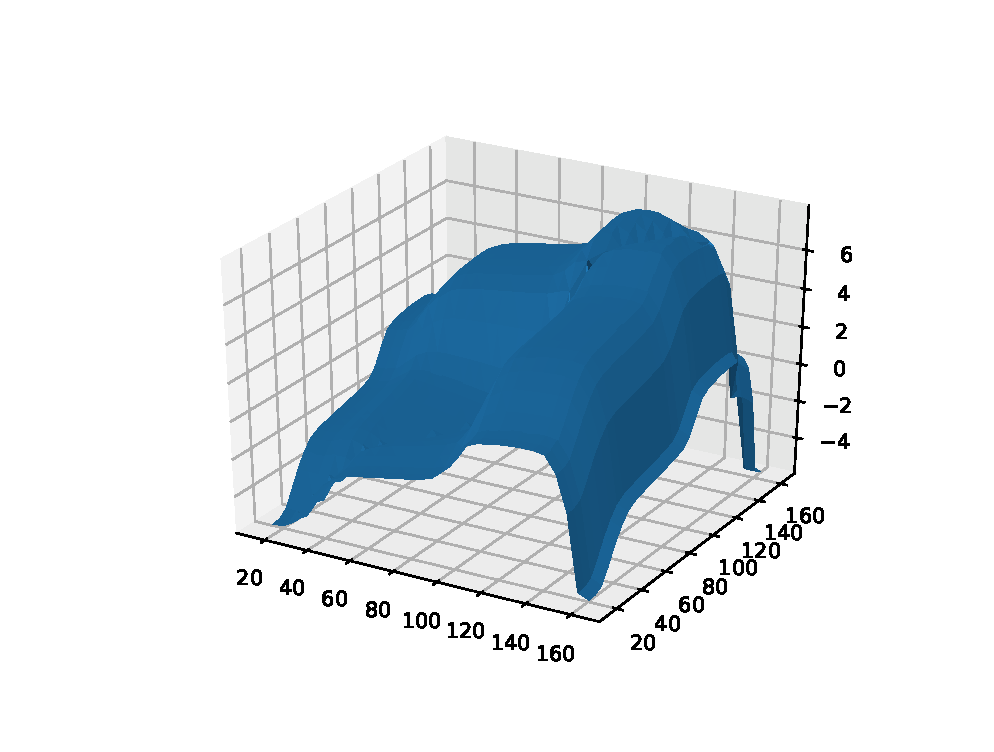
\includegraphics[width=0.4\textwidth]{Im020_1landscape_Kapur.eps}
   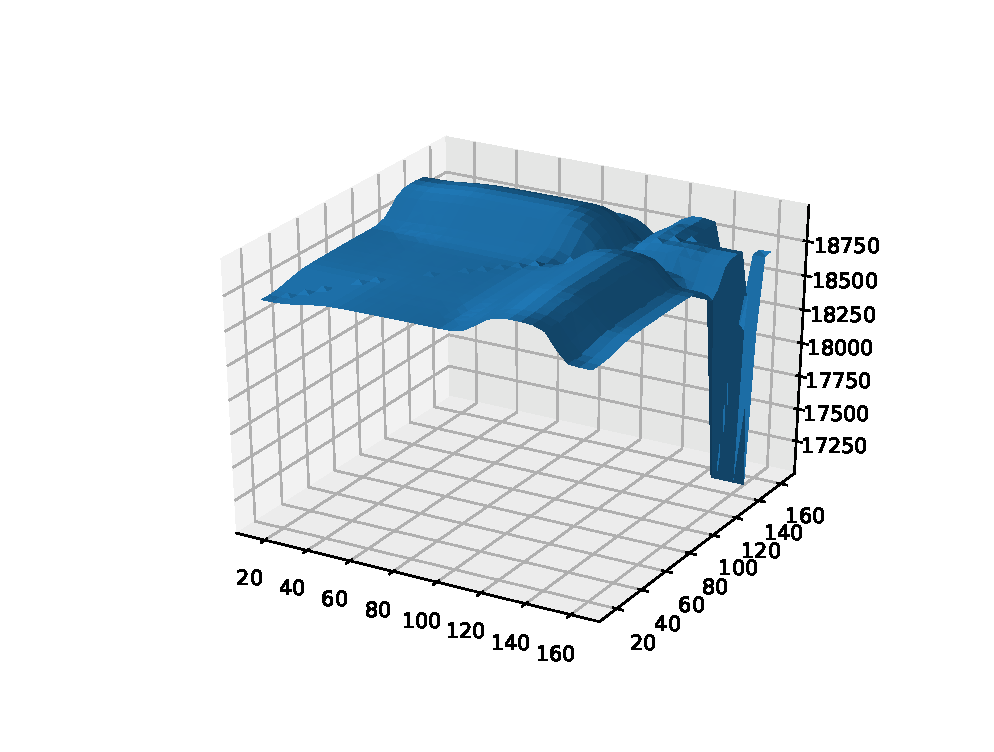
\includegraphics[width=0.4\textwidth]{Im020_1landscape_Otsu.eps} \\
   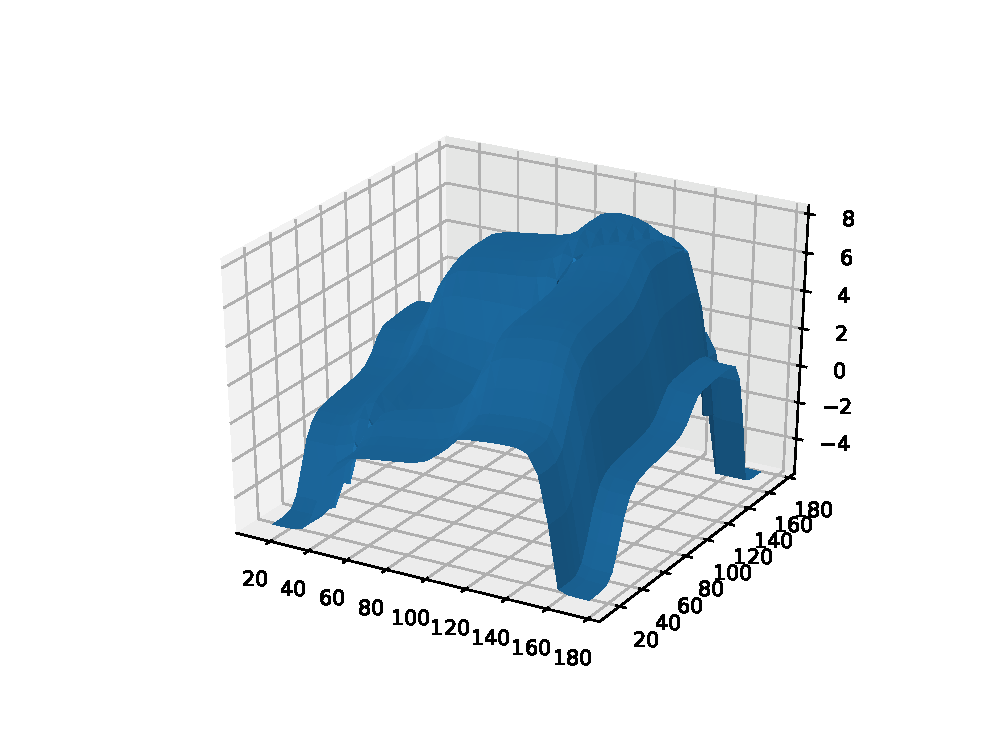
\includegraphics[width=0.4\textwidth]{Im025_1landscape_Kapur.eps}
   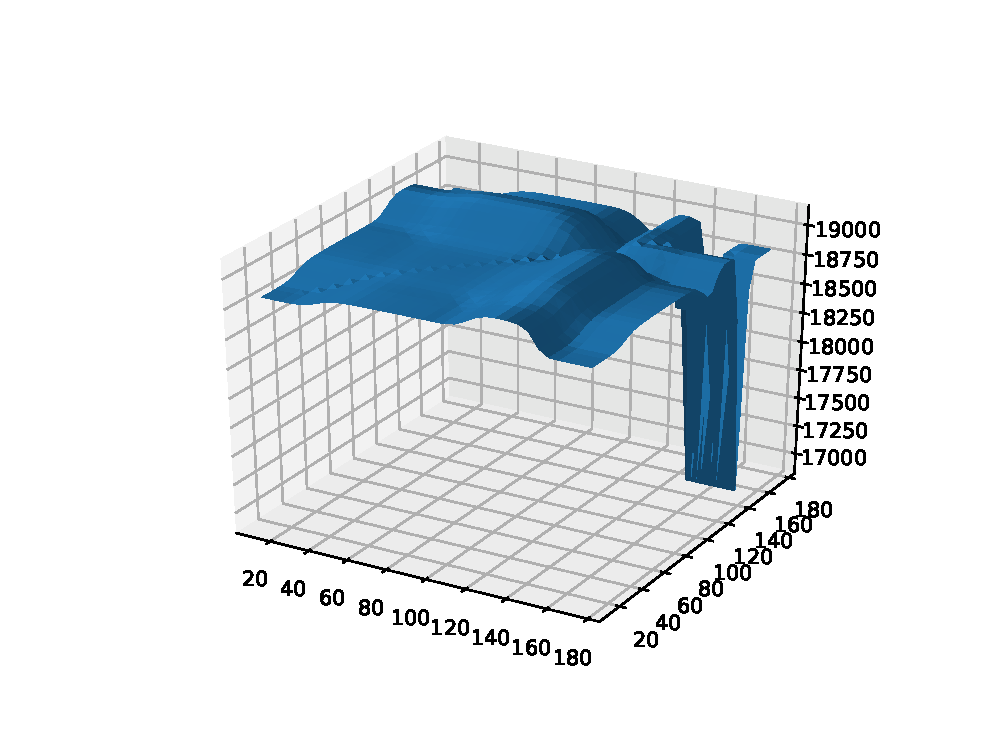
\includegraphics[width=0.4\textwidth]{Im025_1landscape_Otsu.eps}
\end{tabular}
\caption{Función objetivo de la imágen \textit{Im020\_1.jpg} (primer fila) y \textit{Im025\_1.jpg} (segunda fila). En la parte izquierda de cada fila se ilustra la función objetivo de Kapur y en la parte derecha la función objetivo de Otsu.}\label{img:landscape}
\end{figure}

\section{conclusiones}

En este trabajo se estudiaron cinco algoritmos para realizar umbralización de imágenes en escala de grises.
%
Específicamente se  puede concluir los siguiente.
%
\begin{itemize}
 \item El modelo utiliza en el método de Otsu puede sobre-ajustar los parámetros y en resultado no propocionar la mejor segmentación de la imágen.
 \item La propuesta de Evolución Diferencial basado en la función de Otsu obtiene los mismos resultados que el método de Otsu en umbralización de dos y tres niveles.
 \item El método de Otsu considerando más de cuatro niveles no es factible ya que implica un problema de combinatoria.
 \item El método del gradiente basado en la función de Otsu proporciona la mejor exactitud, esto se debe a que el optimizador no proporciona los puntos óptimos y en resultado el model de Otsu no es sobre-ajustado, sin embargo en algunas imágenes el rendimiento de este método es muy malo.
 \item El modelo de Kapur posee propiedades deseables en el ámbito de optimización.
\end{itemize}

Basado en lo que se encontró, se hace énfasis que la parte de modelación del problema tiene un rol muy importante.
%
Una propuesta sencilla conssiste en un modelo el cual esté basado en la combinación lineal del método de Kapur y el método de Otsu, algo similar a lo aplicado en regressión con Lasso y Ridge (Elastic-Net).
%


%%
%% Start line numbering here if you want
%%
\linenumbers

%% main text

%% The Appendices part is started with the command \appendix;
%% appendix sections are then done as normal sections
%% \appendix

%% \section{}
%% \label{}

%% References
%%
%% Following citation commands can be used in the body text:
%% Usage of \cite is as follows:
%%   \cite{key}          ==>>  [#]
%%   \cite[chap. 2]{key} ==>>  [#, chap. 2]
%%   \citet{key}         ==>>  Author [#]

%% References with bibTeX database:

\bibliographystyle{model1-num-names}
\bibliography{sample.bib}

%% Authors are advised to submit their bibtex database files. They are
%% requested to list a bibtex style file in the manuscript if they do
%% not want to use model1-num-names.bst.

%% References without bibTeX database:

% \begin{thebibliography}{00}

%% \bibitem must have the following form:
%%   \bibitem{key}...
%%

% \bibitem{}

% \end{thebibliography}


\end{document}

%%
%% End of file `elsarticle-template-1-num.tex'.
